\chapter{Support Vector Machines (SVM)}
\section{SVM Model}
\par SVM is a supervised learning algorithm, generally used for classification. SVM has been exhaustively used in email spam detection~\cite{2} and image spam detection~\cite{7}. In the training phase SVM constructs a separating hyper-plane. In this section, we give a brief overview of the SVM algorithm.

\par There are 4 key concepts of SVM algorithm as described by Stamp M., in \i{ Machine Learning with Applications in Information Security}~\cite{Stamp_ML}.
\begin{itemize}
	\item \textbf{Separating Hyperplane:} In the training phase, SVM attempts to find a separating hyper-plane which divides labeled input data into two classes. In an ideal scenario, all the data of one class falls on one side of the hyperplane and other class falls on the other side. 
	
	\item \textbf{Maximize Margins:} To construct an optimal hyperplane, only a subset of training data is required. These points are called the support vectors. The idea behind choosing an optimal hyperplane is to maximize the distance/margin between the support vectors of each class and the hyperplane. Fig.\ref{}. shows a separating hyperplane and support vectors for 2D data.
	\begin{figure}[htb]
		\centering
		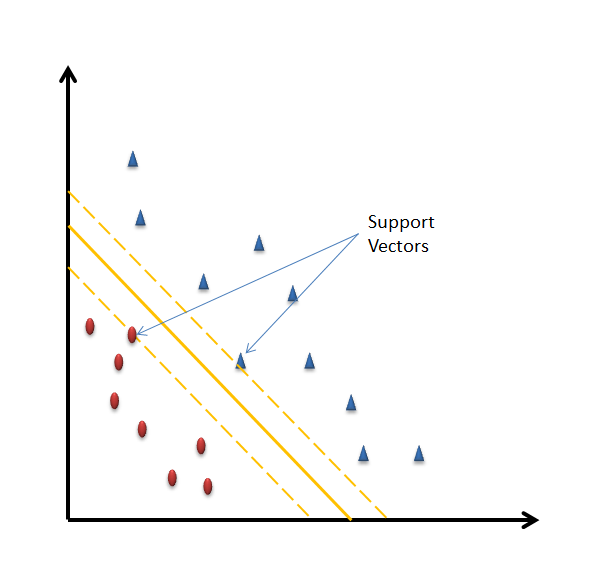
\includegraphics[scale=0.7]{images/svm-hyperplane}
		\caption{Separating Hyper-plane}
		\label{fig:svm_hyperplane}
	\end{figure} 
	
	
	\item \textbf{Work in higher dimensions:} Separating hyperplane is essentially a linear decision function. However, data of the input space is often not linearly separable. Hence, SVM converts the input data to a feature space higher dimension. Input data in this form is more spread out and linearly separable. Hence, classifying data becomes easier. This transformation is however an expensive task.
	
	\item \textbf{Kernel Trick:} Kernel Trick is the mapping function used to transform input space to a linearly separable higher dimension. It makes a non-linear transformation an easy task. It doesn't actually perform the transformation to the higher dimension yet gives us the advantages of working in higher dimensions. Multiple Kernel functions are available like Linear Kernel, Polynomial Kernel, Radial Basis Function(RBF), etc.
	
\end{itemize}
\subsection{Training Phase}

\par Training phase involves generating an equation for the separating hyper plane. It is done by solving a Lagrangian Duality problem. Given a set of input data $X_{0}, X_{1}...., X_{n}$, with labels $z_{0}, z_{1}...., z_{n}$, where $z_{i} \in \{-1, 1\}$, the training phase solves the Lagrangian Duality Problem for Select Kernal function K and C as follows - 
	\[ \text{Maximize } L( \,\lambda) \, = \frac{1}{2} \sum\limits_{i=1}^{n}\sum\limits_{j=1}^{n} \lambda_{i}\lambda_{j} z_{i} z_{j} (X_{i} \cdot X_{j})\] 
	\[\textbf{Subject to constraints } \sum\limits_{i=1}^{n}\lambda_{i}z_{i} = 0 ~and~ C \geq \lambda_{i} \geq 0 ~for~ i=1,2..n.\] 
\subsection{Testing Phase}
\par In the testing phase, we classify a point by determining on which side of the hyperplane the point lies on.

\section{Feature Selection}
\par In a multidimensional  input space, the cost of converting the input space to a higher dimension increases. Though SVM is a classification algorithm, SVM also calculates weights for each feature and ranks them based on their contribution to classification. The idea behind feature selection is reduction of dimensionality. The cost of converting an input space to higher dimension/applying kernel transformations is high. So instead, using the ranks for each feature, we select only top k features for testing phase.


\subsection{Recursive Feature Elimination}

\par Recursive Feature Elimination (RFE) is a feature selection technique used to get rid of the features that contribute the least to SVM classification. Here, we use RFE to fine tune the SVM classification for unraveling ham and spam images. RFE assigns weights to features and ranks them according to the amount of contribution towards the classification. The feature with the least rank is eliminated and the process is repeated till the desired number of features are eliminated. RFE works only with Linear Kernel of SVM.

\subsection{Univariate Feature Selection}
\par Univariate feature selection uses univariate statistical properties to rank each feature. The top k ranked features are then selected.

\section{Scoring Metrics}
\par When any data point is scored, the result is one of the following 4 outcomes- 
\begin{enumerate}
	
	\item True Positive(TP): The scored sample is a spam, and it is rightly classified as spam.
	\item True Negative(TN): The scored sample is a ham, and it is rightly classified as ham.
	\item False Positive(FP): The scored sample is ham, and it is wrongly classified as spam.
	\item False Negative(FN): The scored sample is spam, and it is wrongly classified as ham.
\end{enumerate} 
\par In the real world, we want to reduce the FP rate as low as possible and increase TP and TN. We measure SVM scores in the form of accuracy. Accuracy can be defined as- 
\[ \textbf{Accuracy} =  \frac{TP+TN}{P+N} \]
where P = total positive samples and N = total negative samples.

\subsection{Confusion Matrix}
\par Confusion Matrix visualizes the four cases for given dataset. Fig. \ref{fig:confusionMatrix}. shows a confusion matrix.

\begin{figure}
	\centering
	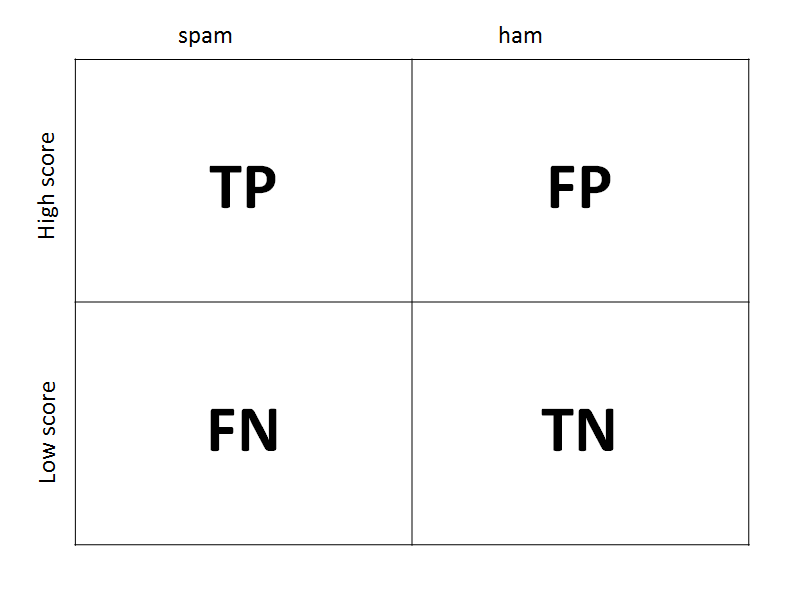
\includegraphics[width=0.5\linewidth]{images/confusionMatrix}
	\caption{Confusion Matrix}
	\label{fig:confusionMatrix}
\end{figure}


\subsection{Receiver Operating Characteristic(ROC) Curve}
\par For any binary classifier, ROC curve is constructed by plotting True Positive Rate(TPR) versus False Positive Rate(FPR) for varying threshold values. True Positive Rate(TPR) is also called sensitivity, True Negative Rate(TNR) is also called specificity. FPR = 1 - specificity. TPR and TNR can be defined as follows- 
\[ \textbf{TPR} =  \frac{TP}{TP+FN}  \textbf{  and   TNR} =  \frac{TN}{TN+FP}    \]

\par Area Under the Curve (AUC) for an ROC is used as a scoring metric. An AUC of 1.0 is perfect accuracy and AUC of 0.5 is like flipping a coin. Fig. \ref{fig:rocCurve}. shows an example of an ROC curve.


\begin{figure}
	\centering
	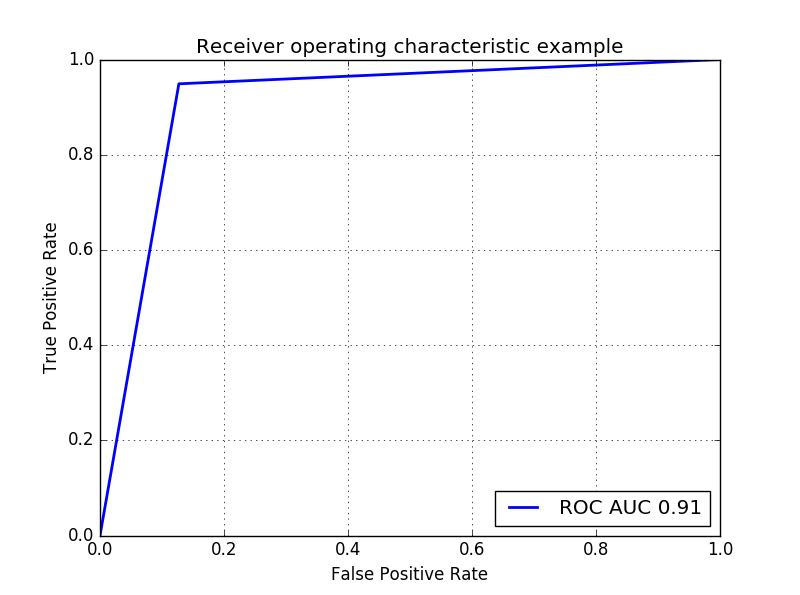
\includegraphics[width=0.5\linewidth]{images/rocCurve}
	\caption{ROC Curve}
	\label{fig:rocCurve}
\end{figure}
